\section{Auswertung}
\label{sec:Auswertung}

\begin{table}[!htp]
\centering
\caption{Die Daten der Amplitudenmessung bei der gedämpften Schwingung.}
\label{tab:zeit-amplitude}
\begin{tabular}{S[table-format=3.0] S[table-format=1.2]}
\toprule
{$t$ / µs} & {$U$ / V} \\
\midrule
14 & 8.16 \\
27 & 6.80 \\
41 & 5.92 \\
54 & 4.96 \\
68 & 4.40 \\
81 & 3.60 \\
95 & 3.20 \\
108 & 2.72 \\
122 & 2.32 \\
136 & 2.00 \\
149 & 1.68 \\
162 & 1.44 \\
176 & 1.28 \\
189 & 1.12 \\
203 & 0.96 \\
217 & 0.80 \\
\bottomrule
\end{tabular}
\end{table}

\begin{figure}
    \centering
    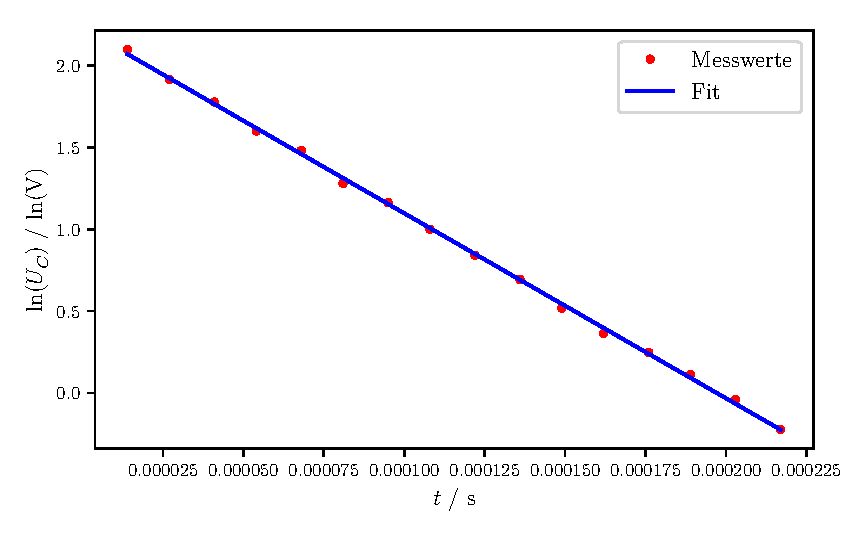
\includegraphics{build/plot-amplitude.pdf}
    \label{fig:zeit-amplitude}
    \caption{Plot und Fit der Messwerte der Messung der Amplitude in Zeitabhängigkeit.}
\end{figure}

\begin{center}
    $a = (1.131 \pm 0.008) \cdot 10^{4} \frac{\ln(\symup{V})}{\symup{s}}$

    $b = (2.23 \pm 0.01) \ln(\symup{V})$
\end{center}

%%%%%%%%%%%%%%%%%%%%%%%%%%%%%%%%%%%%%%%%%%%%%%%%%%%%%%

\begin{table}[!htp]
\centering
\caption{Die angegebenen Gerätedaten.}
\label{tab:geraetedaten}
\begin{tabular}{S[table-format=1.2] @{${}\pm{}$} S[table-format=1.2] S[table-format=1.3] @{${}\pm{}$} S[table-format=1.3] S[table-format=2.1] @{${}\pm{}$} S[table-format=1.1] S[table-format=3.1] @{${}\pm{}$} S[table-format=1.1]}
\toprule
\multicolumn{2}{c}{$L$ / mH} & \multicolumn{2}{c}{$C$ / nF} & \multicolumn{2}{c}{$R_1$ / $\symup{\Omega}$} & \multicolumn{2}{c}{$R_2$ / $\symup{\Omega}$} \\
\midrule
3.53 & 0.03 & 5.015 & 0.015 & 30.3 & 0.1 & 271.6 & 0.3 \\
\bottomrule
\end{tabular}
\end{table}

Errechneter $R_\text{ap}$ Wert

\begin{center}
    $R_\text{Theorie} = (1677 \pm 8)$ $\symup{\Omega}$ 
\end{center}

Gemessener Wert

\begin{center}
    $R_\text{ap} = (1355 \pm 5)$ $\symup{\Omega}$
\end{center}

%%%%%%%%%%%%%%%%%%%%%%%%%%%%%%%%%%%%%%%%%%%%%%%%%%%%%%

\begin{table}[!htp]
\centering
\caption{Die Amplituden und Phasenverschiebung in Frequenzabhänigkeit mit $U_0 = 6.55$ V.}
\label{tab:var-freq}
\begin{tabular}{S[table-format=2] S[table-format=2.1] S[table-format=1.2]}
\toprule
{$f$ / kHz} & {$U_C$ / V} & {$\Delta t$ / µs} \\
\midrule
12 & 7.2 & 1.2 \\
14 & 7.8 & 1.5 \\
16 & 8.1 & 1.5 \\
18 & 8.3 & 1.6 \\
20 & 9.0 & 1.7 \\
22 & 9.5 & 1.8 \\
24 & 10.3 & 2.2 \\
26 & 11.3 & 2.5 \\
28 & 12.4 & 2.9 \\
30 & 13.8 & 3.4 \\
32 & 15.2 & 4.2 \\
33 & 16.0 & 4.6 \\
34 & 16.5 & 5.1 \\
35 & 16.8 & 5.6 \\
36 & 16.8 & 6.3 \\
37 & 16.5 & 6.8 \\
38 & 15.9 & 7.3 \\
39 & 15.1 & 7.7 \\
40 & 14.2 & 8.0 \\
41 & 13.2 & 8.2 \\
42 & 12.2 & 8.3 \\
44 & 10.5 & 8.5 \\
46 & 9.0 & 8.5 \\
48 & 7.5 & 8.4 \\
50 & 6.5 & 8.28 \\
52 & 5.7 & 8.08 \\
54 & 5.1 & 7.84 \\
56 & 4.6 & 7.72 \\
58 & 4.1 & 7.48 \\
60 & 3.7 & 7.28 \\
62 & 3.4 & 7.08 \\
\bottomrule
\end{tabular}
\end{table}

\begin{figure}
    \centering
    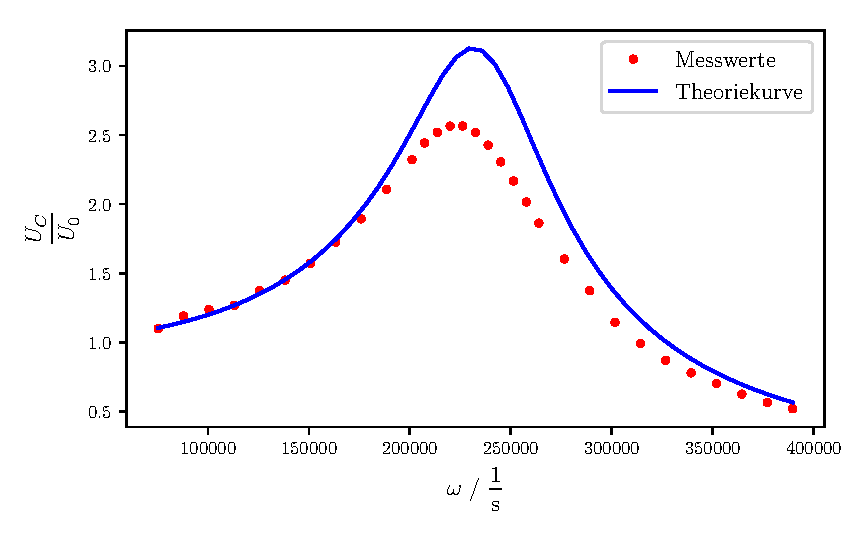
\includegraphics{build/plot-guete.pdf}
    \label{fig:guete}
    \caption{Plot und Theoriekurve des Amplitudenverhältnis gegen die Frequenz aufgetragen.}
\end{figure}

\begin{center}
    $q_\text{exp} = 2.56$
\end{center}

\begin{center}
    $q_\text{theo} = 3.09 \pm 0.01$
\end{center}

\begin{equation}
    \Delta q_\text{theo} = \sqrt{\cdot \frac{L}{C}} \cdot \sqrt{ \bigg( \frac{1}{R^2} \Delta R \bigg)^2 + \bigg(\frac{1}{2RC} \Delta L \bigg)^2 + \bigg(\frac{L}{2RC^2} \Delta C \bigg)^2}
\end{equation}

\begin{center}
    $\omega_+ = (2.79 \pm 0.01) \cdot 10**{5}$ $\frac{1}{s}$

    $\omega_- = (2.022 \pm 0.008) \cdot 10**{5}$ $\frac{1}{s}$
\end{center}

Der Fehler nach Gauß errechnet sich dabei nach

\begin{equation}
    \Delta \omega_{+,-} = \sqrt{\bigg( \frac{\partial \omega_{+,-}}{\partial C} \cdot \Delta C \bigg)^2 + \bigg( \frac{\partial \omega_{+,-}}{\partial L} \cdot \Delta L \bigg)^2 + \bigg( \frac{\partial \omega_{+,-}}{\partial R} \cdot \Delta R \bigg)^2}, 
\end{equation}

wobei die einzelnen partiellen Ableitungen im Folgenden aufgeführt sind:

\begin{center}
    $\bigg( \frac{\partial \omega_{+,-}}{\partial C} \bigg)^2 = \Bigg( \dfrac{1}{2L\sqrt{\frac{1}{LC}+\frac{R^2}{4L^2}}C^2} \Bigg)^2$

    $\bigg( \frac{\partial \omega_{+,-}}{\partial R} \bigg)^2 = \Bigg( \dfrac{R}{4L^2\sqrt{\frac{R^2}{4L^2}+\frac{1}{CL}}} \pm \dfrac{1}{2L} \Bigg)^2$

    $\bigg( \frac{\partial \omega_{+,-}}{\partial L} \bigg)^2 = \Bigg( \mp \dfrac{R}{2L^2}+\dfrac{-\frac{1}{CL^2}-\frac{R^2}{2L^3}}{2\sqrt{\frac{1}{CL}+\frac{R^2}{4L^2}}} \Bigg)^2$.
\end{center}

\begin{figure}
    \centering
    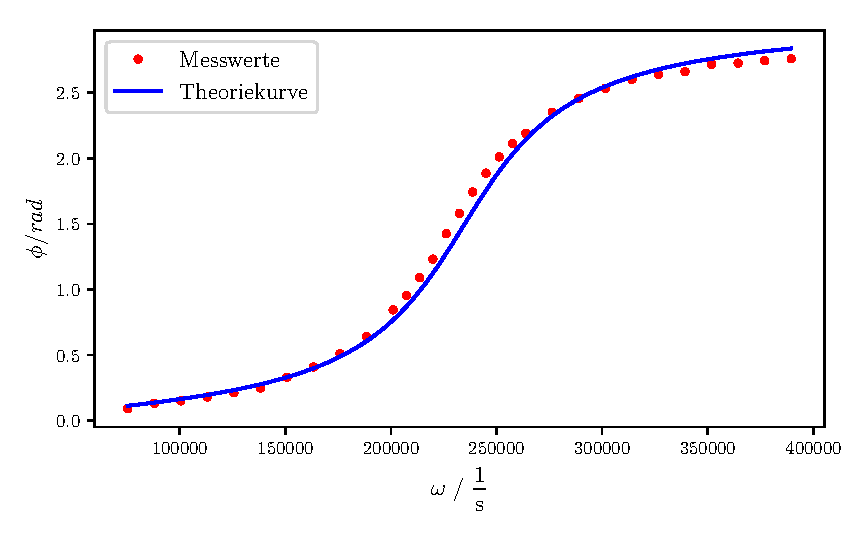
\includegraphics{build/plot-phase.pdf}
    \label{fig:phase}
    \caption{Plot und Theoriekurve des Phasenunterschiedes gegen die Frequenz aufgetragen.}
\end{figure}
